\section{Fitnessfunktion}
\begin{frame}{Fitnessberechnung}
    \begin{columns}[T] % T aligns the tops of the columns
        \begin{column}{0.75\textwidth}
            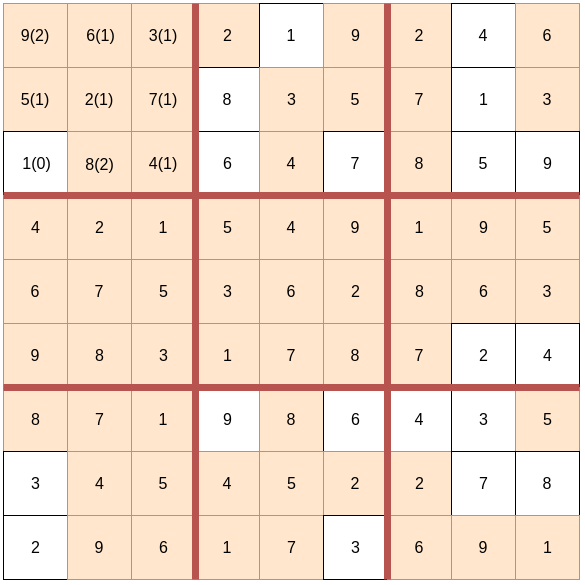
\includegraphics[width=\textwidth]{Pictures/Collision-Fitness.png}
        \end{column}
        \begin{column}{0.35\textwidth}
            \begin{itemize}
                \item Kollisionszahl als Fitnesswert (=86)
                \item Speicherung individueller Werte für Zellen \\
                (s. Block 0)
            \end{itemize}
            Andere Idee für Fitnessberechnung:
            \begin{itemize}
                \item \(|\sum_{i=0}^{9}i-\sum_{i=0}^{9}x_{ij}|\) (Zeile0 \(\rightarrow\) 3)
                \item \(|9!-\prod_{i=0}^{9}x_{ij}|\) (Zeile0 \(\rightarrow\) 222912)
                \item \(|\{1,2,...,9\}\setminus \{x_{0j},x_{1j},...,x_{8j}\}|\) (Zeile0 \(\rightarrow\) 3)
            \end{itemize}
        \end{column}
    \end{columns}
\end{frame}
